%
% results.tex
%
% Copyright (C) 2018 by Andre Martins Pio de Mattos <andrempmattos@gmail.com>.
%
% Internship Report
%
% This work is licensed under the Creative Commons Attribution-ShareAlike 4.0
% International License. To view a copy of this license,
% visit http://creativecommons.org/licenses/by-sa/4.0/.
%

%
% \brief Title page.
%
% \author Andre Martins Pio de Mattos <andrempmattos@gmail.com>
%
% \version 0.1.0
%
% \date 08/09/2019
%

\newpage

\section{Results} \label{sec:results}

In order to accomplish the payload mission, several simulation, tests and verification were performed. In this document only the most important tests are presented and detailed.

%--------------------------------------------------------------------------------

\subsection{Subsystem Tests}

In order to validate the first concepts, a simulation before the design synthesis was performed intending to verify mainly the SDRAM controller. The Microsemi development tool (Libero) has integration with ModelSim (a simulation software) and provide the Bus Functional Model (BFM) solution, which enables the emulation of the communication between MSS and fabric logic through the AHB. The \autoref{fig:simulation_flow} demonstrates the simulation flow using the BFM scripts. The user defines the commands in the BFM script, then a compiler converts them to a vector file that is further used as an input for the testbench system, which consists of an AHB master interface, the memory controller, and the emulated memory. Since the memory controller is part of the Microsemi catalog, the sources of this testbench scheme are provided to support the early design validation. For this simulation, the script performed explicit write and read operations successively, leaving the task of setup and refresh commands to the memory controller, since it must independently execute this operations.

\begin{figure}[!ht]
    \begin{center}
        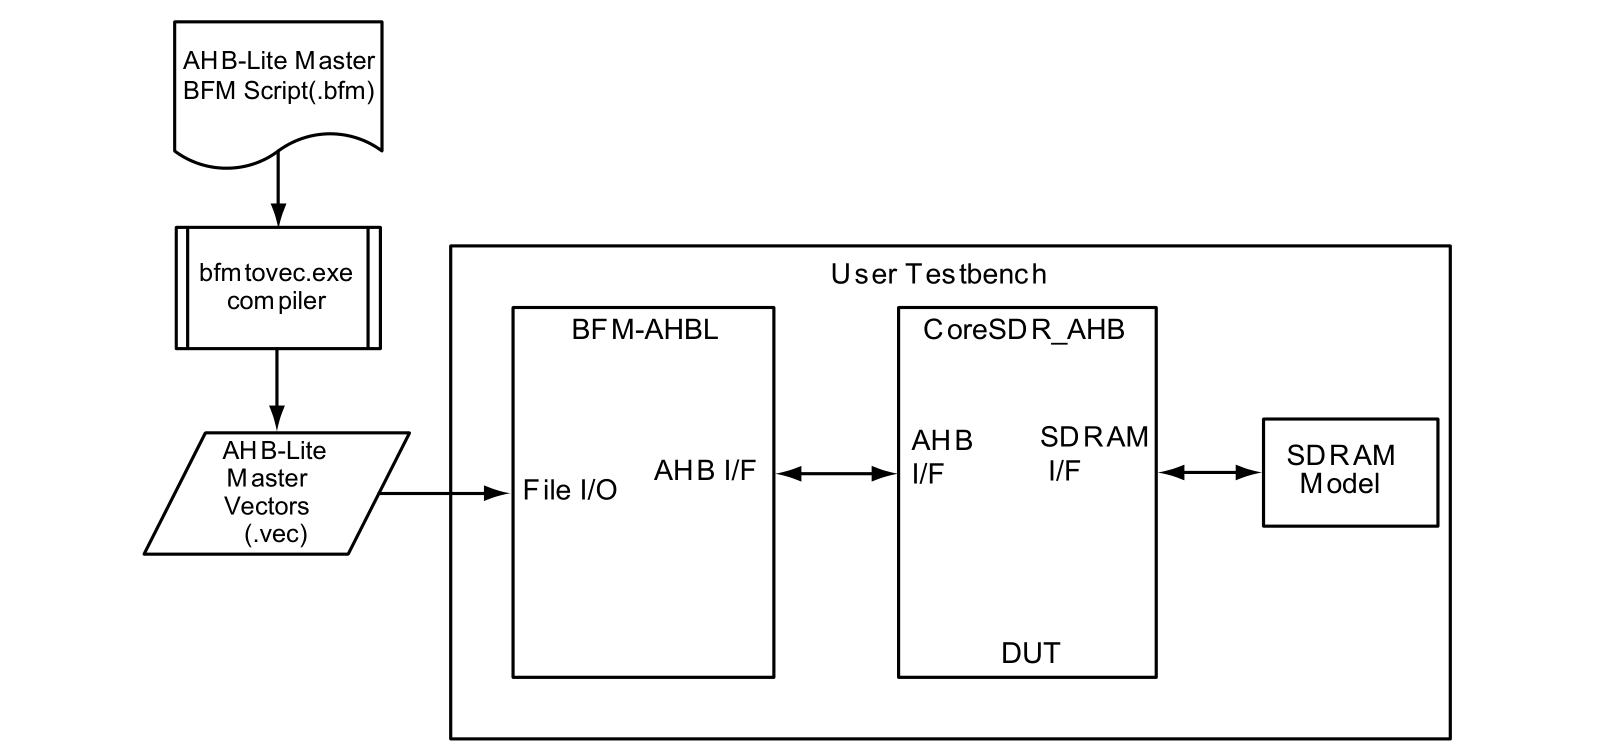
\includegraphics[width=0.9\textwidth]{figures/flow_simulation.png}
        \caption{Memory controller simulation flow.}
        \label{fig:simulation_flow}
    \end{center}
\end{figure}

The \autoref{fig:simulation_controller} shows a part of the simulation execution, regarding refresh, load mode, read and write commands. The parameters were selected in conformity with the datasheet nominal values.

\begin{figure}[!ht]
    \begin{center}
        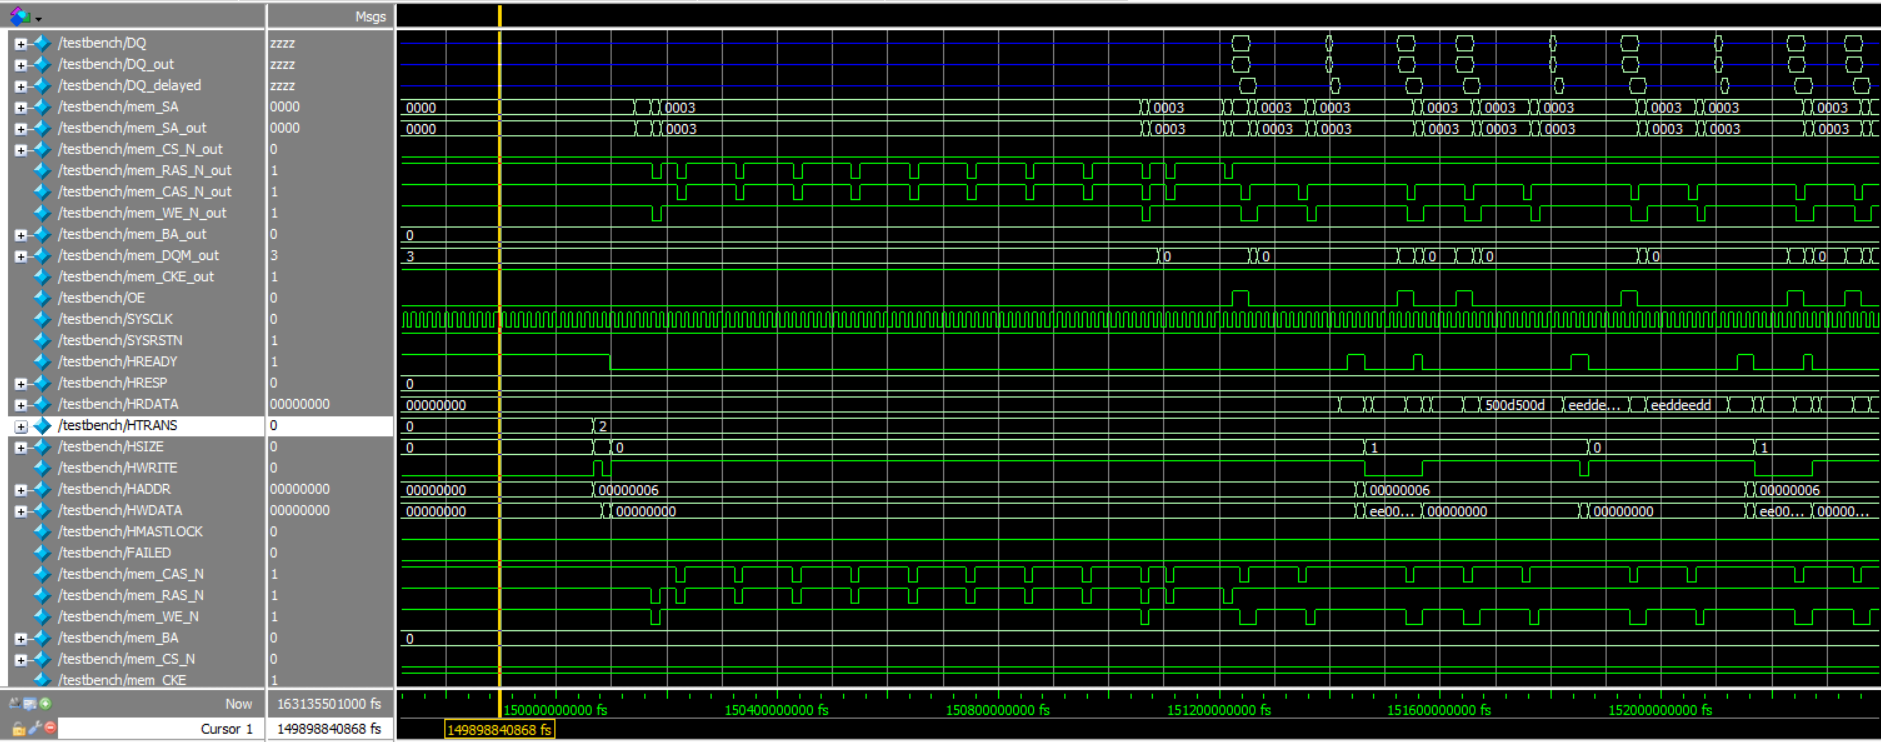
\includegraphics[width=\textwidth]{figures/simulation_controller.png}
        \caption{Memory controller simulation results.}
        \label{fig:simulation_controller}
    \end{center}
\end{figure}

During this design evaluation, some misunderstanding of memory parameters were detected and corrected, such as the refresh rate that was smaller than the minimal recommended. Also, this test ensured that the memories could operate in parallel without losing the timing constraints and functional requirements.

%--------------------------------------------------------------------------------

\subsection{System Tests}

During the development and improvements for the flight model, it was possible to evaluate the payload under experimental radiation conditions. Two identical boards were exposed to high energy neutrons during continuous hours before presenting critical damage and reported several events. This experiment allowed improvements in the design (adjustments of the memory controller parameters for this abnormal conditions) and presented some limitations, since this type of radiation was not the main target of the experiment due to high energy exposure. As presented in \autoref{fig:setup-test-rad}, the payload (mentioned as "HARSH") was one of the several experiments performed in this test campaign.     

\begin{figure}[!ht]
    \begin{center}
        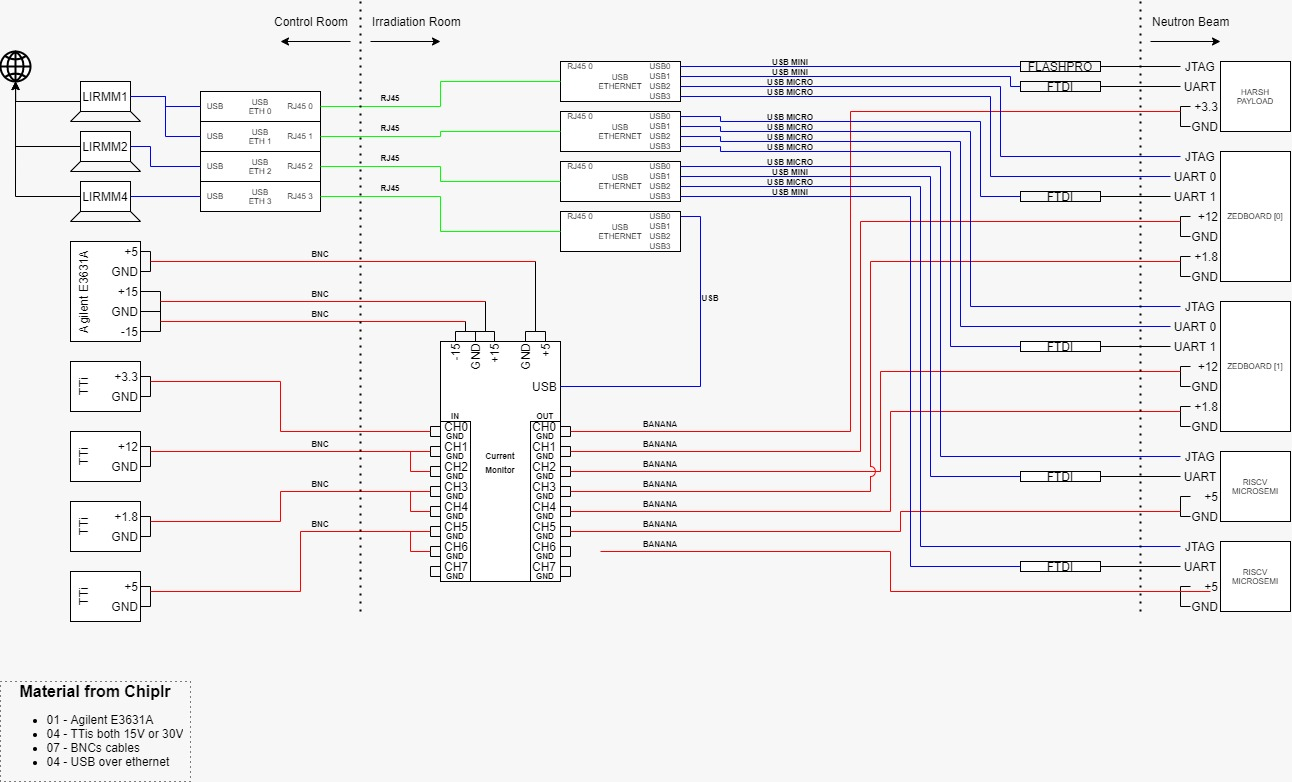
\includegraphics[width=0.9\textwidth]{figures/setup_test_rad.jpeg}
        \caption{Radiation experiment setup (high energy neutrons beam).}
        \label{fig:setup-test-rad}
    \end{center}
\end{figure}

The \autoref{fig:log_test_rad} shows a log message example for this type of test. During the experiment, several log messages were generated and analysed to evaluate performance under radiation and produce actual radiation events, which represents the closest test setup in earth for the payload in the orbit. In this particular log it is possible to detected that there is an error in the last address of the SDRAM memory model B after performing consecutive write and read operations. Since the time difference between operations is too short, in this case there was any event detected despite the one error detected. This error is injected in the last address to verify if in that execution the algorithm is running correctly, since under radiation the device might present some defects.  

\begin{figure}[!ht]
    \begin{center}
        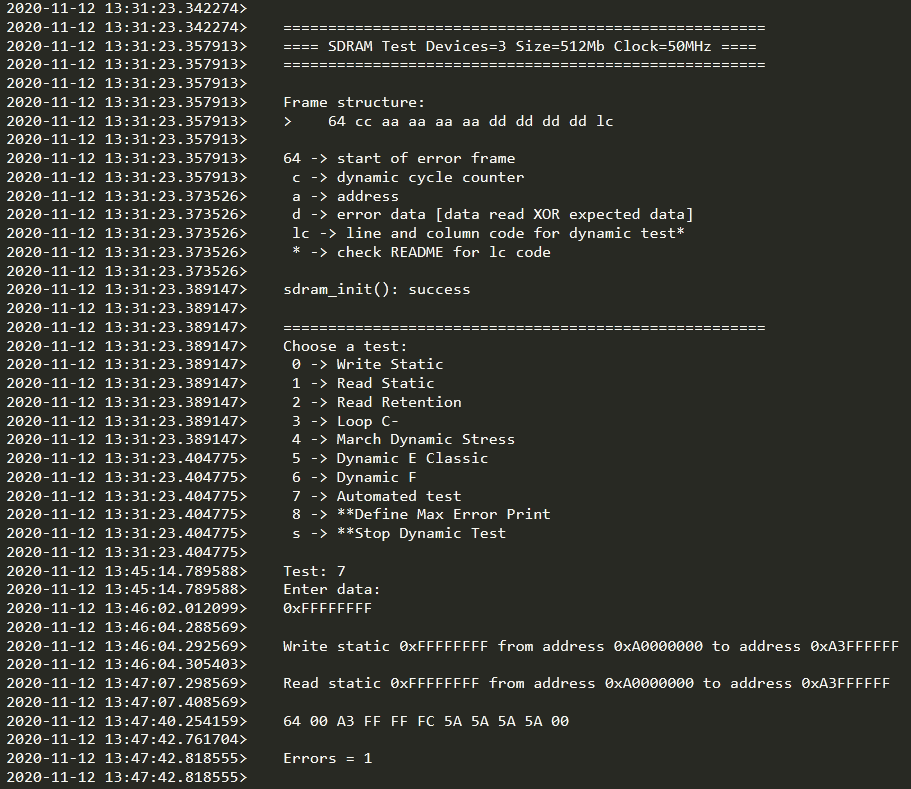
\includegraphics[width=0.85\textwidth]{figures/log_test.png}
        \caption{Log message example during the radiation tests.}
        \label{fig:log_test_rad}
    \end{center}
\end{figure}


%================================================================================

\subsection{System Integration}

The payload was tested using different methods and configurations to achieve its stability and reliability. The first assessments started during the simulations for the memory chips using the ModelSim simulator. Then, the design was validated in the development kit through static tests in its SDRAM memory and due to similar behavioral characteristics from the memories studied in this work, it was possible to evaluate and measure important characteristics of the implementation. After this preliminary tests, using the engineering model, the payload was tested in conjunction with the OBDH and its functional operation was validated. The flight model was assessed alongside the entire satellite system and later qualified for flight. These steps are described in details in the following sections, starting with the engineering model integration since the previous stages were presented across the document.  

The integration with the engineering model occurred in three different steps: the first using a Raspberry Pi as OBC, the second with an older version of the GOLDS-UFSC OBDH (the FloripaSat-I OBDH), and the last using the GOLDS-UFSC OBDH engineering model. In order to perform the first tests, a Raspberry Pi 3 was used to emulate the OBC behavior and communication. This approach was necessary due to limited access to the actual OBDH. Despite the hardware differences, this test setup allowed the debug of the most critical communication issues and the improvement of the interface protocol.

The \autoref{fig:sig_cmd_in} presents a command request from the OBC during tests of the first stage. It is important to note that the communication between the payload and the OBC uses the FloripaSat Protocol (FSP). In the figure is shown 8 bytes: header, destination address, source address, package type, number of paylaod packages, payload (command in this case) and the last two for CRC.

\begin{figure}[!ht]
    \begin{center}
        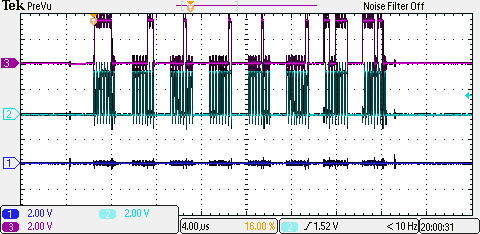
\includegraphics[width=1\textwidth]{figures/fsp_cmd_in.png}
        \caption{Example SPI command communication signals from the OBC to the payload using the FSP protocol.}
        \label{fig:sig_cmd_in}
    \end{center}
\end{figure}

The \autoref{fig:sig_ack_out} presents the payload acknowledgement answer due to the master request. The same package structure is observed, differing just for the type, payload content, address positions, and CRC check.  

\begin{figure}[!ht]
    \begin{center}
        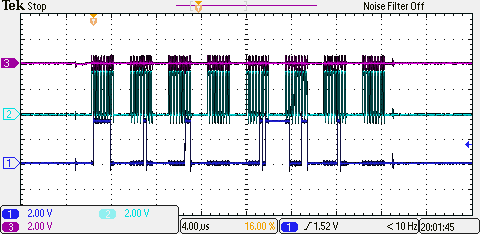
\includegraphics[width=1\textwidth]{figures/fsp_ack_out.png}
        \caption{Example SPI acknowledgement answer communication signals from the OBC to the payload using the FSP protocol.}
        \label{fig:sig_ack_out}
    \end{center}
\end{figure}

%--------------------------------------------------------------------------------



\clearpage